
\chapter{Implementierung}
\label{chapter-implementierung}
Das folgende Kapitel beschreibt die Implementierung des Reservierungsinterfaces sowie des Frontends.
Zunächst werden die Implementierung des Reservierungsinterfaces und die damit einhergehenden
technischen Aspekte beschrieben (\ref{subsec:aufbauinterface}). Dabei wird Aufschluss über die
Struktur gegeben und die Kernfunktionalitäten (\ref{subsec:kernfkt}) sowie Herausforderungen
(\ref{subsec:heraus}) in der Realisierung näher erläutert. Daraufhin wird die Umsetzung des
Frontends erläutert (\ref{subsec:frontend}). Abschließend wird auf die Inbetriebnahme des Systems
eingegangen (\ref{subsec:nutzung}).

\section{Implementierung des Reservierungsinterfaces}
\label{sec:interface}
Dieser Abschnitt erläutert den technischen Aufbau des Rervierungsinterfaces und geht auf relevante
Aspekte in der Realisierung der Kernfunktionalitäten (\ref{section:funktionale}) ein. Des Weiteren
werden unerwartete Herausforderungen thematisiert, welche im Rahmen der Arbeit nicht bewältigt
werden konnten.


\subsection{Aufbau des Reservierungsinterface}
\label{subsec:aufbauinterface}
Das Reservierungsinterface teilt sich in drei wesentliche Bestandteile: der
\textit{Fastify-HTTP-Server}, die \textit{SQLite Datenbank} und das \textit{ORM Prisma} (vgl.
\ref{fig:level3}). Diese Komponenten spiegeln sich auch in der Verzeichnisstruktur aus \ref{fig:db}
wider.
\begin{figure}[h]
  \centering
  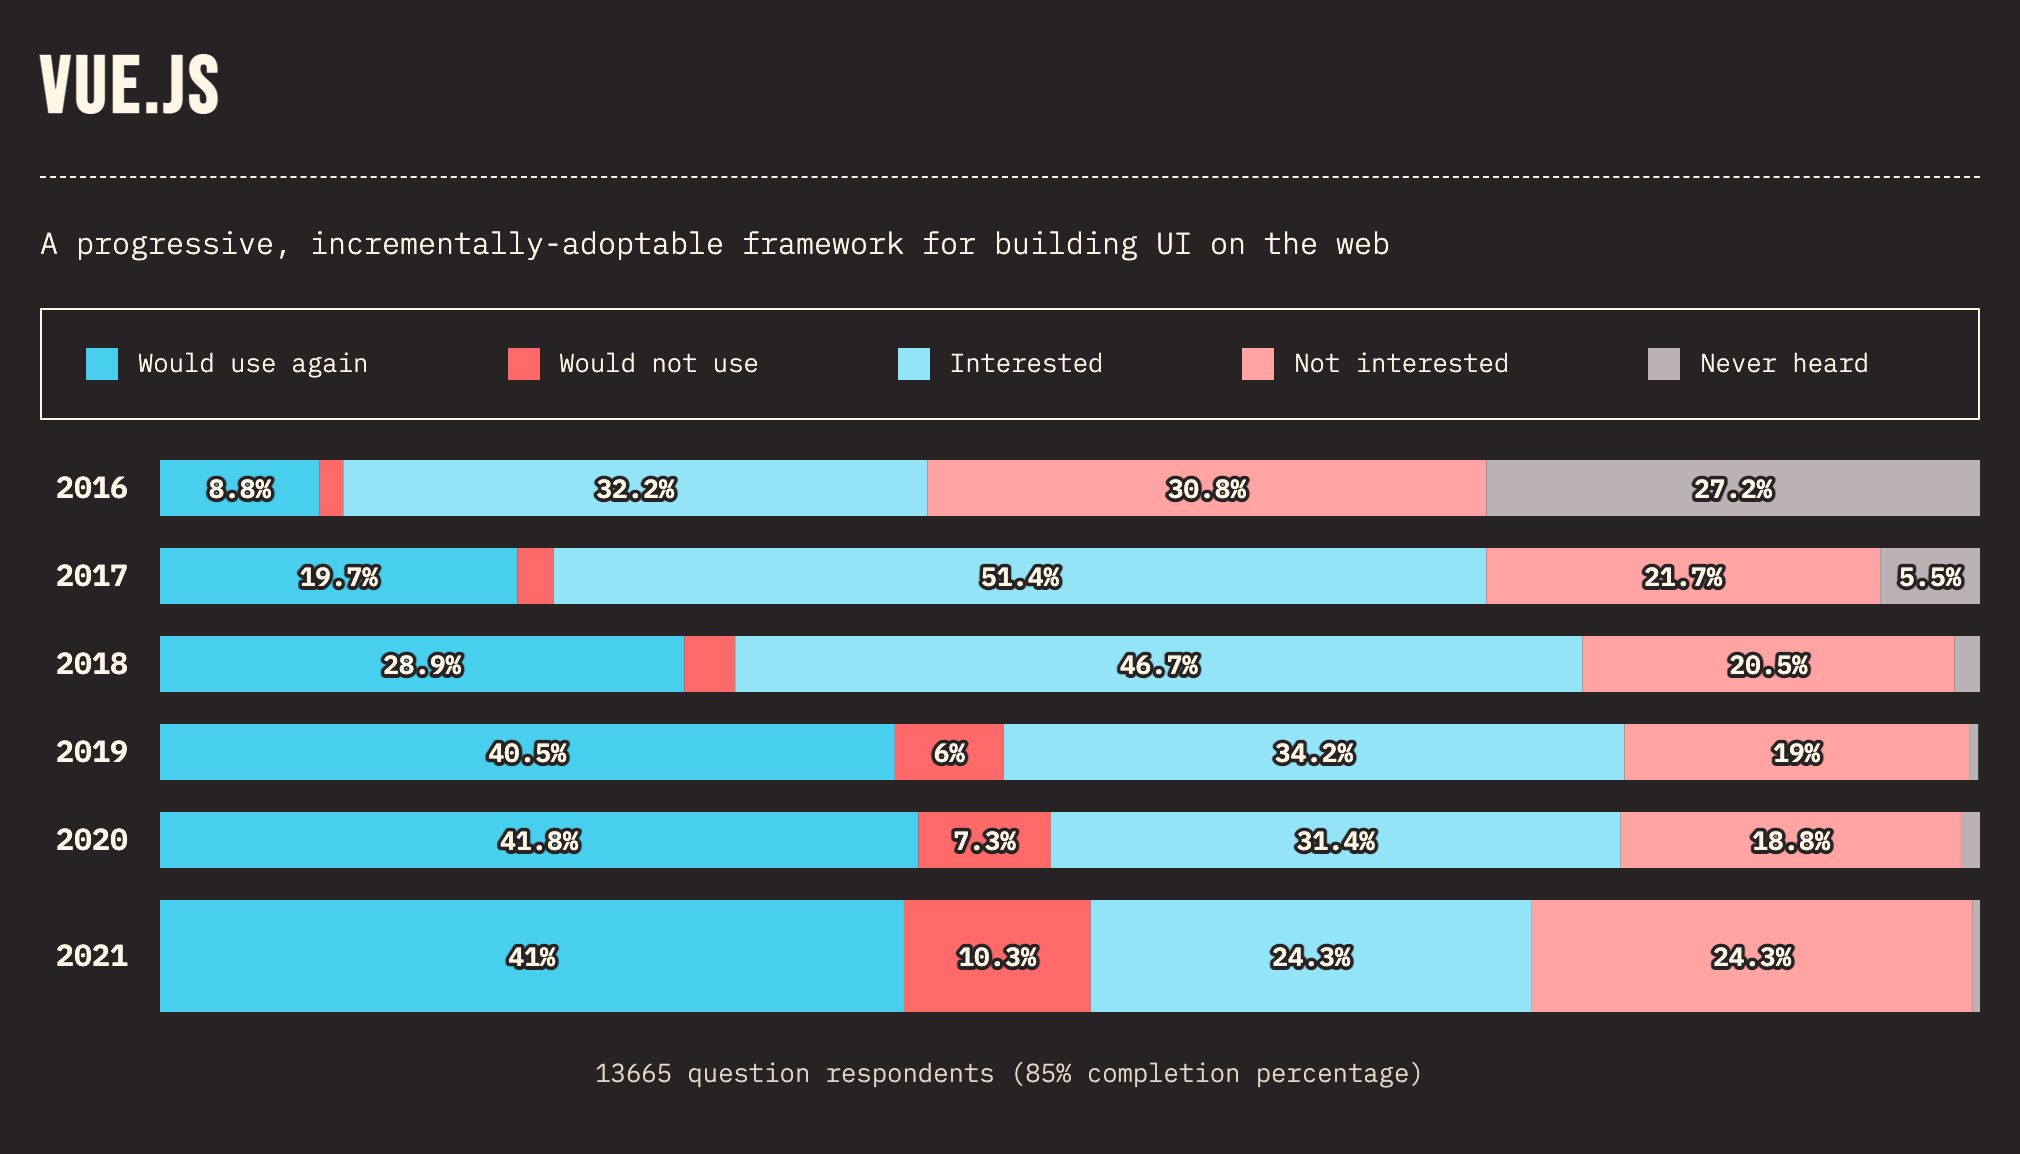
\includegraphics[scale=0.2]{Bilder/vuejs.png}
  \caption[Verzeichnisstruktur des Reservierungsinterfaces]{Verzeichnisstruktur des Reservierungsinterfaces}
  \label{fig:db}
\end{figure}
Der HTTP-Server findet sich in der \textit{server.ts} wieder und stellt dort die API des
Reservierungsinterfaces bereit. Die entwickelte API lässt sich in drei Bereiche teilen:
\textit{Assets}, \textit{Kategorien} und \textit{Reservierungen} (\ref{table:impl-backend-routes}).
Für die drei Inhaltstypen werden die Routen aus \ref{table:impl-backend-routes} bereitgestellt,
welche die von \citeA{fielding_hypertext_2014} beschriebene Semantik für HTTP-Methoden beachten.
Folglich werden bei Verwendung der \textit{GET}-Methode ausschließlich Daten zurückerhalten.
Hingegen muss bei einer Anfrage mit zu übermittelnden Daten die \textit{POST}-Methode verwendet
werden, um einen neuen Eintrag im System zu erschaffen. Beispielsweise wird eine
\textit{GET}-Anfrage an \textit{/assets/:id} abgeschickt, um die Informationen eines Assets zu
erhalten. Um den Status in Snipe-IT auf \textit{herausgegeben} zu aktualisieren, wird eine
\textit{POST}-Anfrage an \textit{/reservation/receive} gesendet, sobald Verleihende eine abgeholte
Reservierung bestätigen.
\begin{table}[h]
  \centering
  \caption{API des Reservierungsinterfaces}
  \begin{tabular}{lll}
    \arrayrulecolor{maincolor}\hline
    \sffamily\color{maincolor}Methode & \sffamily\color{maincolor}Route &
    \sffamily\color{maincolor}Funktion                                                              \\
    \arrayrulecolor{maincolor}\hline
    GET                               & \textit{/assets}                & Erhalte alle Assets       \\
    GET                               & \textit{/assets/:id}            & Erhalte ein Asset mit der
    entsprechende ID                                                                                \\
    GET                               & \textit{/categories}            & Erhalte alle Kategorien   \\
    GET                               & \textit{/reservation}           & Erhalte Reservierungen    \\
    POST                              & \textit{/reservation}           & Erstellen Reservierung    \\
    POST                              & \textit{/reservation/receive}   & Erstellen Reservierung    \\
    POST                              & \textit{/reservation/return}    & Erstellen Reservierung    \\
    POST                              & \textit{/reservation/id}        & Erstellen Erstellen
    Reservierung                                                                                    \\
    DELETE                            & \textit{/reservation/delete}    & Löschen Reservierungen    \\
    PATCH                             & \textit{/reservation/patch}     & Verändern Reservierung    \\
    \arrayrulecolor{maincolor}\hline
  \end{tabular}
  \label{table:impl-backend-routes}
\end{table}

Die mit SQLite bereitgestellte Datenbank speichert die Reservierungen sowie die
Profile. Hierfür wurde das in \ref{fig:orm} dargestellte Datenbankschema
erarbeitet. Zur Umsetzung dieses Schemas wurde das ORM Prisma genutzt, welches
drei zentrale Funktionen bietet (\ref{fig:prisma}).
\begin{figure}[h]
  \centering
  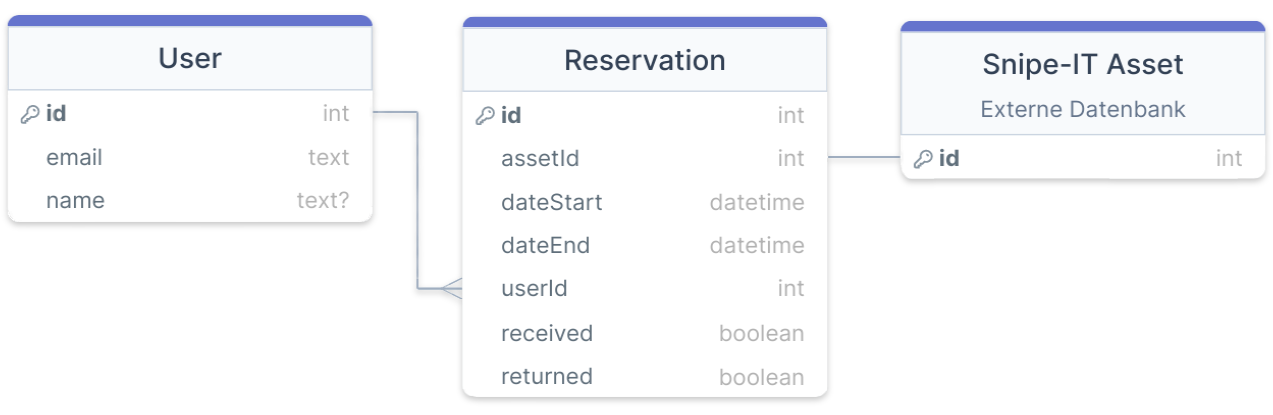
\includegraphics[scale=0.35]{Bilder/Code/UML_DB.png}
  \caption[Datenstruktur der Reservierungen in Verbindung mit Nutzenden]{Datenstruktur der Reservierungen in Verbindung mit Nutzenden}
  \label{fig:orm}
\end{figure}

\begin{enumerate}
  \item Beschreibung des Schemas durch eigene \ac{dsl}
  \item Automatisierte Migration bei Schemaänderung
  \item JavaScript-Client mit generierten TypeScript-Typen
\end{enumerate}

\begin{figure}[p]
  \centering
  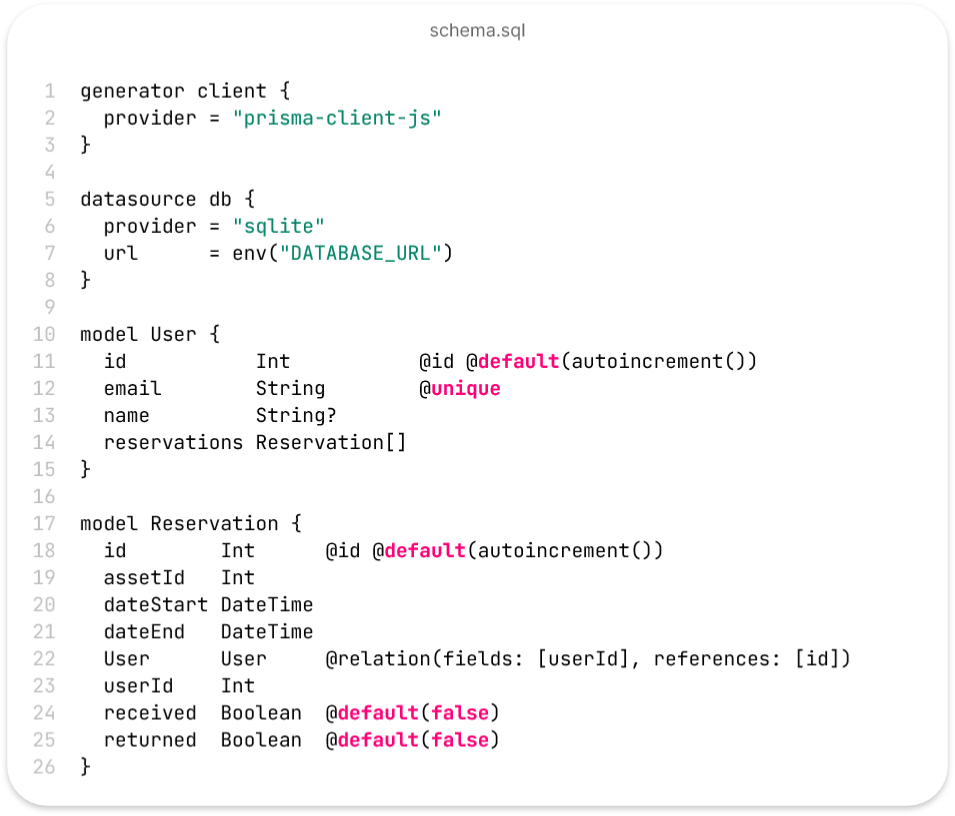
\includegraphics[scale=0.35]{Bilder/Code/schemasql.png}
  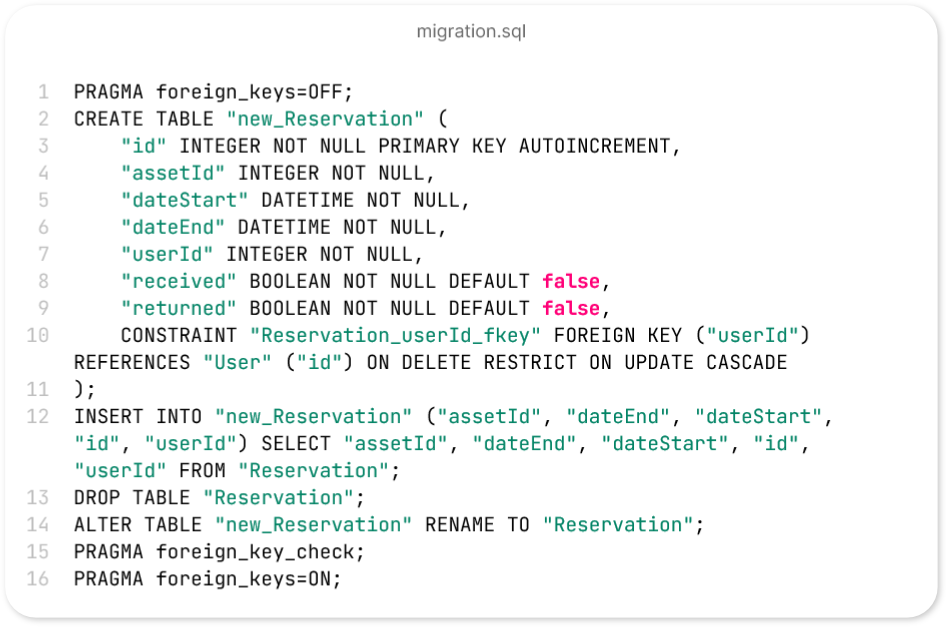
\includegraphics[scale=0.35]{Bilder/Code/migrationsql.png}
  \caption[Quellcode: schema.prisma und migration.sql]{Quellcode: schema.prisma und migration.sql}
  \label{fig:prisma}
\end{figure}


\subsection{Implementierung der Kernfunktionalität}
\label{subsec:kernfkt}
Dieser Abschnitt präsentiert die Implementierung der Kernfunktionalität des
Reservierungsinterfaces, welche aus den Anforderungen bestimmt wurde (\ref{section:anforderung}).
Bei der Funktionalität handelt es sich um das Reservieren in die Zukunft, sowie das Speichern
dieser Vorgänge und die damit einhergehende Bestätigung für die Aktualisierung in Snipe-IT.


Sobald ein Asset über die Web-App ausgeliehen wird, werden die relevanten Daten mit einer
\textit{POST}-Anfrage an die \textit{/reservation}-Route des Reservierungsinterfaces gesendet.
Diese relevanten Daten (Assetname, Datum, Uhrzeit, Ort, etc.) werden im Reservierungsinterfaces
gespeichert. Sobald Verleihende die Ausleihe bestätigen, wird der Ausleihstatus mit einer
\textit{POST}-Anfrage an \textit{/reservation/receive} intern und in Snipe-IT von
\textit{ausleihbar} zu \textit{herausgegeben} aktualisiert. Zur Kommunikation zwischen dem
Reservierungsinterface und Snipe-IT wird das Paket \textit{node-fetch} genutzt, welches die
Fetch-API des Browsers in \textit{Node.js} bereitstellt. Für das Aktualisieren des Status eines
Assets mit der \textit{assetId} wird beispielsweise eine \textit{POST}-Anfrage an
\textit{<SnipeIt\_URL>/api/v1/hardware/<assetId>/checkout} versendet, welche die ID des
\textit{herausgegeben}-Status und die ID des ausleihenden Nutzenden beinhaltet (\ref{fig:server}).
Analog geschieht dies für das Zurückgeben eines Assets mit einer \textit{POST}-Anfrage an
\textit{/reservation/return}.
\begin{figure}[h]
  \centering
  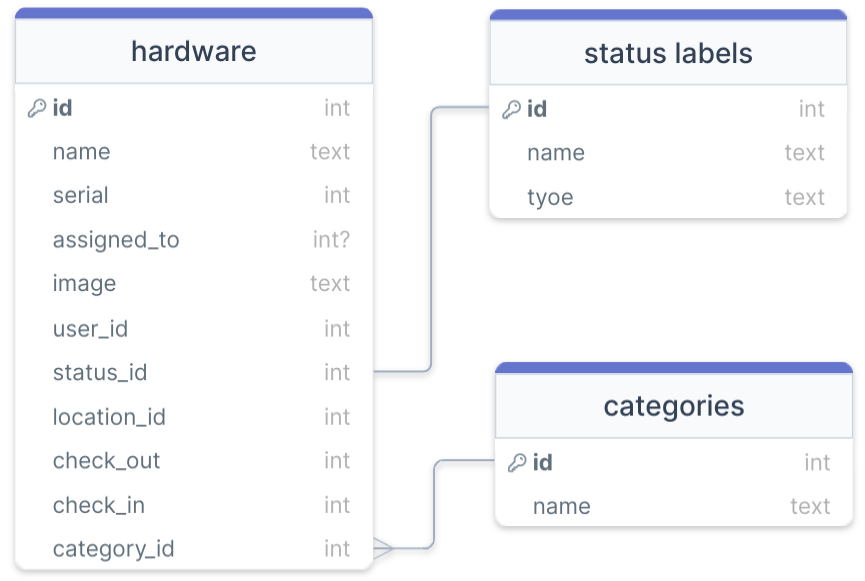
\includegraphics[scale=0.4]{Bilder/Code/DB_RES_INT.png}
  \caption[UML Snipe-IT API]{UML Snipe-IT API}
  \label{fig:server}
\end{figure}

Um auf die Assets zugreifen zu können, wurde mit der Snipe-IT JSON REST API gearbeitet. Die Snipe-IT
API umfasst viele Routen\footnote{\url{https://snipe-it.readme.io/reference/api-overview}} für die
Abfrage und Manipulation der internen Datenbank, wovon \textit{/hardware, /categories} und
\textit{/statuslabels} relevant für die Umsetzung dieser Arbeit waren. \ref{fig:snipe} zeigt den
Aufbau und die Beziehungen der genutzten Snipe-IT API Ressourcen, wobei die Ressource
\textit{hardware} den Assets in der Snipe-IT Datenbank entspricht.
\begin{figure}[h]
  \centering
  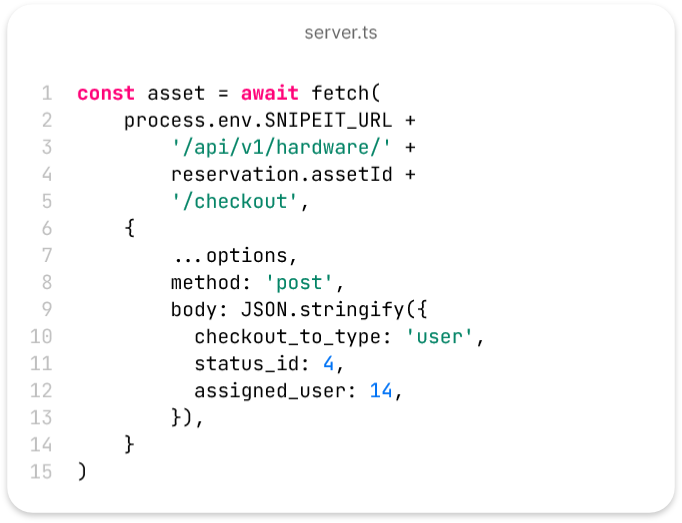
\includegraphics[scale=0.4]{Bilder/Code/serverts.png}
  \caption[Quellcode: server.ts]{Quellcode: server.ts}
  \label{fig:snipe}
\end{figure}

Um mit der API arbeiten zu können, muss ein \textit{persönliches
  Zugriffstoken}\footnote{\url{https://snipe-it.readme.io/reference/generating-API-tokens}} für die
Nutzung generiert werden. Das persönliche Zugriffstoken muss mit jeder Anfrage an die API, in Form
eines \lstinline{Bearer <Token>} HTTP-Headers, mitgeschickt werden. Da persönliche Zugriffstoken
verwendet werden, spiegeln die Berechtigungen des API-Tokens die Berechtigungen des Nutzenden
wider.

\subsection{Herausforderungen in der Einbindung von LDAP}
\label{subsec:heraus}
Snipe-IT bietet bereits eine integrierte Lösung zur Synchronisation und Login mit
LDAP\footnote{\url{https://snipe-it.readme.io/docs/ldap-sync-login}}. Da die \textit{persönlichen
  Zugriffstoken} jedoch die einzige Authentifizierungsmöglichkeit der API sind und lediglich manuell
im Dashboard generiert werden können, kann das LDAP-System der Universität zu Lübeck nicht ohne
Umstände eingebunden und entsprechend genutzt werden.

Ein möglicher Lösungsansatz wäre das programmatische Nutzen eines Browsers aufseiten des
Reservierungsinterfaces, welcher die Angaben von Nutzenden in der Wep-App verwendet, um mit diesen
den LDAP-Login in Snipe-IT durchzuführen. Sollte der Snipe-IT Login erfolgreich sein, könnten
Nutzende für den Rest der Sitzung als authentifiziert gelten. Im Reservierungsinterface selbst
würde ein speziell für das Reservierungsinterface generierte Token für die Kommunikation mit
Snipe-IT genutzt werden.

\section{Implementierung des Frontends}
\label{subsec:frontend}
Das kommende Kapitel beschreibt die Client-seitige Realisierung der Arbeit. Zunächst wird der Aufbau
betrachtet, daraufhin wird auf das Extrahieren der Unterkategorien eingegangen (\ref{fig:vue}).


Für den Aufbau des Projektes wurde aus den in \ref{chapter-konzept} festgestellten Anforderungen
\textit{vue.js} verwendet. Bei der Implementierung wurde sich an den best practices der
Vue.js-Dokumentation orientiert \todo{(Vue.js, 2021a)}. Für sich wiederholende Elemente wurden
eigene Views erstellt. Dadurch ergibt sich eine hierarchisch geschachtelte Client-Anwendung der
Vue-Komponenten. \ref{fig:vue} stellt die Komponenten-Struktur vereinfacht dar. Um
konkretere Vorschläge in der Entwicklungsumgebung zu ermöglichen und vorzeitige Fehler zu
minimieren, wurde ergänzt zu \textit{JavaScript} \textit{TypeScript} verwendet.

\subsection{Aufbau der Routen und Komponentenstruktur}
Für die Realsisierung der Routen wurde der File-Based-Routing Ansatz verwendet, welcher die Routen
aufgrund der Verzeichnisstruktur generiert. Hierfür wurde das Vite-Plugin
\textit{vite-plugin-pages}\footnote{\url{https://github.com/hannoeru/vite-plugin-pages}} genutzt.
Vue-Komponenten, welche sich im \textit{/pages}-Verzeichnis des Projekts befinden, werden in eine,
dem Dateinamen gleichende, Route umgewandelt. Ordner können hierbei verwendet werden, um Unterrouten
zu erstellen, während die Verwendung von eckigen Klammern zur Kennzeichnung von Parametern genutzt
wird. Beispielsweise wird eine \textit{[id].vue}-Datei, welche sich in dem Ordner
\textit{categories} befindet, in die \textit{/categories/<id>}-Route umgewandelt, welche die
angegebene ID in der Komponente als Parameter nutzen kann (\ref{fig:vue}).
\begin{figure}[h]
  \centering
  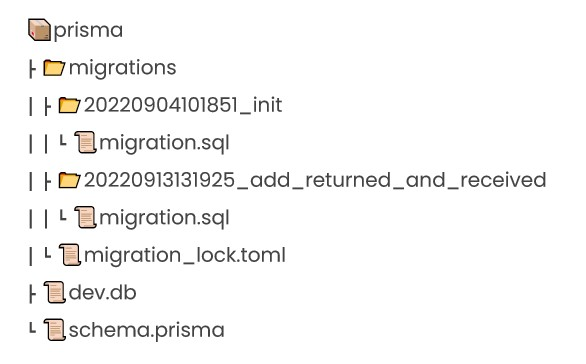
\includegraphics[scale=0.7]{Bilder/Db.jpg}
  \caption[Verzeichnisstruktur des Clients]{Verzeichnisstruktur des Clients}
  \label{fig:vue}
\end{figure}

\subsection{Extrahieren von Unterkategorien}
Die im Rahmen dieser Arbeit verwendete Beispieldatenbank beinhaltete eine Vielzahl an Kategorien und
Unterkategorien welche nach folgendem Format benannt wurden: \enquote{Kategorie - Unterkategorie}.
Das verwendete Format ergibt sich aus der fehlenden Funktionalität Snipe-Its, einem Asset mehrere
Kategorien zuweisen zu können. Da das Anzeigen der Kategorien in diesem Format unübersichtlich ist,
sollten zunächst nur die Oberkategorien und anschließend die Unterkategorien angezeigt werden.
\ref{fig:categoriecode} stellt eine vereinfachte Form des verwendeten Quellcodes dar.
\begin{figure}[h]
  \centering
  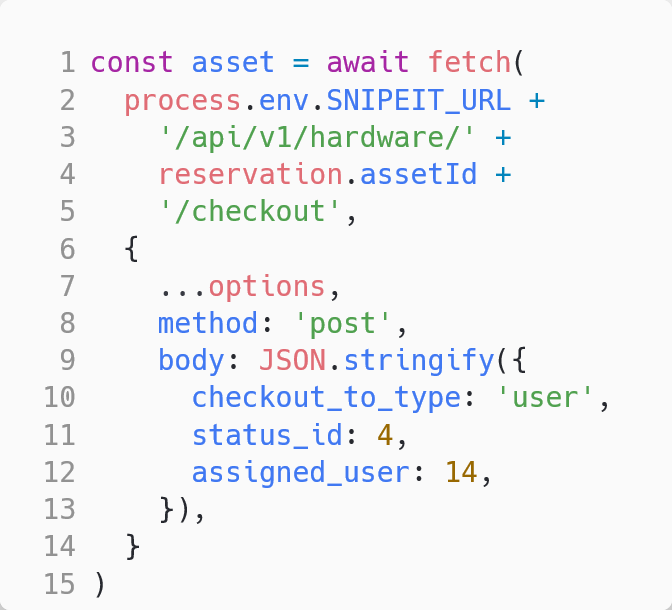
\includegraphics[scale=0.4]{Bilder/carbon(1).png}
  \caption[vereinfachte Form des verwendeten Quellcodes]{vereinfachte Form des verwendeten Quellcodes}
  \label{fig:categoriecode}
\end{figure}

Zur Extrahierung werden die erhaltenen Kategorien, anhand eines Trennsymbols (\enquote{-}), in Ober- und
Unterkategoriepaare getrennt. Anschließend werden alle Paare mit der gleichen Oberkategorie zu einem
Eintrag zusammengefasst, welcher alle zugehöhrigen Unterkategorien beinhaltet. Hierbei wird für jede
Unterkategorie die hinterlegte Kategorie-ID gespeichert. Somit ergibt sich eine Baumstruktur, welche
in der Anwendung schrittweise durchlaufen werden kann.


\section{Nutzung des Systems}
\label{subsec:nutzung}
Der folgende Abschnitt führt die nötigen Schritte auf, um das System in Betrieb nehmen zu können.
Zuerst wird die Installation erklärt, gefolgt von der Konfiguration und Ausführung des Systems.

\subsection{Installation}
Für die Nutzung des Systems wird eine Installation von \textit{Node.js} vorausgesetzt. Zunächst
müssen alle eingebundenen Pakete des \textit{npm} Paketverzeichnis mit \lstinline{npm install}
installiert werden. Dies muss für Server (\lstinline{\server}) und Client (\lstinline{\client})
jeweils im entsprechenden Verzeichnis ausgeführt werden. Zusätzlich sollte die Datenbank im
Server-Verzeichnis mithilfe des Befehls \lstinline{npx prisma install }\todo{Befehl raussuchen}
erstellt und vorbereitet werden. Abschließend sollte \lstinline{npx prisma generate} ausgeführt
werden, um die benötigten Datein des Prisma-Clients zu generieren.

\subsection{Konfiguration}
Zur Festlegung von umgebungsabhängigen Variablen werden für Server und Client je eine
\textit{.env}-Datei verwendet. Diese müssen vor der Inbetriebnahme angelegt werden und sind nach dem
Schema in BILD aufgebaut. Der Server benötigt die URL der zu verwendenden Snipe-IT Instanz, den
API-Key zur Authentifizierung (\ref{section:api}) und den Pfad der SQLite Datenbankdatei.
Aufseiten des Clients wird lediglich die URL des Reservierungsinterfaces benötigt.
\begin{figure}[h]
  \centering
  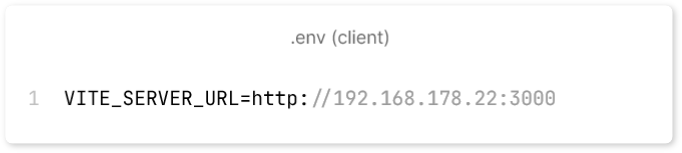
\includegraphics[scale=0.3]{Bilder/Code/client.png}
  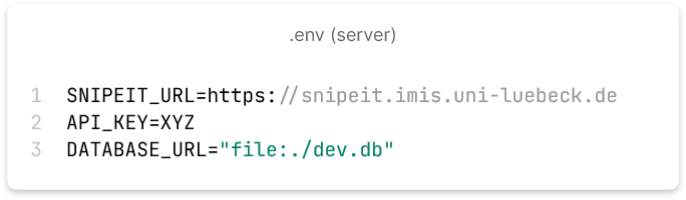
\includegraphics[scale=0.3]{Bilder/Code/sever.png}
  \caption[Inhalte der .env Datei im Frontend (links) und Backend (rechts)]{Inhalte der .env Datei im Frontend (l) und Backend (r)}
  \label{fig:env}
\end{figure}


\subsection{Einrichtung des Snipe-IT API-Zugangs}
\label{section:api}
Um die gewünschte(n) Datenbank(en) aus Snipe-IT nutzen zu können, wird ein Account in Snipe-IT
benötigt, welcher von Administrierenden angelegt werden muss. Daraufhin muss über die
Profileinstellung \textit{Manage API Keys} ein API-Key generiert werden. Der generierte API kann nun
in der Konfiguration genutzt werden. Außerdem sollte beachtet werden, dass der API Key nur einmalig
nach der Generierung einsehbar ist.

\subsection{Ausführung des Reservierungsinterfaces}
Um die Daten der Snipe-IT Datenbank abzurufen, die Reservierungen zwischen zu speichern und den
Status in \textit{Snipe-IT} aktualisieren zu können, muss das Reservierungsinterface mithilfe des
Befehls \lstinline{npm run serve} gestartet werden.


\subsection{Ausführung der Web-App}
Das \enquote{Bauen} der Web-App geschieht über den Befehl \lstinline{npm run build-only}. Nachdem
der Prozess erfolgreich abgeschlossen ist, sollte ein neues \textit{dist}-Verzeichnis generiert
worden sein. Das \textit{dist}-Verzeichnis kann zum statischen Hosting genutzt werden. Zur lokalen
Entwicklung kann durch\lstinline{npm run dev} zudem ein Entwicklungsserver gestartet werden.

\section{Fazit der Implementierung}

Die in der Implementierung realisierten Funktionalitäten umfassen das \textit{muss} der in der
\nameref{section:anforderung} erarbeiteten Funktionen.

Im Rahmen der vorliegenden Arbeit wurde ein umfassendes System realisiert, welche die Grundlagen des
Reservierens mit einer Verknüpfung zu Snipe-IT ermöglicht. Die Implementierung teilt sich in zwei
Teile, dass Reservierungsinterface (Backend) und das Frontend, die Web-App. Das
Reservierungsinterface teilt sich in drei wesentliche Bestandteile: der
\textit{Fastify-HTTP-Server}, die \textit{SQLite Datenbank} und das \textit{ORM Prisma} (vgl.
\ref{fig:level3}). Diese Komponenten spiegeln sich in der Verzeichnisstruktur aus \ref{fig:db}
wider. Für die serverseitige Umsetzung wurde eine API entwickelt, welche sich in drei Bereiche teilt
(\textit{Assets}, \textit{Kategorien} und \textit{Reservierungen} (\ref{table:impl-backend-routes}).
Die Datenbank speichert die getätigten Reservierungen und Beispiel Profile. Für eine vereinfachte
Umsetzung wurde das ORM Prisma verwendet. Die Implementierung der Kernfunktionalitäten zeigt die
Nutzung der Snipe-IT Datenbank. Für die Nutzung dieser musste ein \textit{persönliches
Zugriffstoken} generiert werden. Sobald ein Asset über die Web-App ausgeliehen wird, werden die
relevanten Daten mit einer \textit{POST}-Anfrage an die \textit{/reservation}-Route des
Reservierungsinterfaces gesendet. Diese relevanten Daten werden im Reservierungsinterfaces
gespeichert. Sobald Verleihende die Ausleihe bestätigen, wird der Ausleihstatus mit einer
\textit{POST}-Anfrage an \textit{/reservation/receive} intern und in Snipe-IT aktualisiert. Die
Accoutbasierte Nutzung mit dem LADp-System stelltsich aufgrund des \textit{persönliches
Zugriffstoken} als Herausforderung heraus und wurde demzufolge nicht eingearbeitet. Für den zweiten
Teil der Anwendung wurde \textit{vue.js} und \textit{TypeScript} verwendet. Für den Aufbau der
Routen wurde der File-Based-Routing Ansatz verwendet, welcher die Routen aufgrund der
Verzeichnisstruktur generiert. Hierfür wurde das Vite-Plugin
\textit{vite-plugin-pages}\footnote{\url{https://github.com/hannoeru/vite-plugin-pages}} genutzt.
Abschliend musste eine Extrahierung der Unterkategorien anhand eines Trennsymbols (\enquote{-}),
implementiert werden. 